\documentclass{article}
\author{Jake Lane}
\title{Optimising Higgs Decay events to Background events in the di-photon channel}
\usepackage{amsmath, graphicx, listings	}
\graphicspath{{/Users/jakelane/higgs/figures/}}

\begin{document}
\maketitle
\begin{abstract}
A Higgs decay in to 2 photons ($H \rightarrow \gamma \gamma$) is optimised against a background of 2 photons simulated by python as gluon decay into 2 photons ($g \rightarrow \gamma \gamma$.) The signal was optimised via filtering the events based on their kinematic variables. A strong peak was found at $m = 123 GeV/c^2$ with deviation from the modelled background of $\sigma = $ at the $x$ \% confidence limit.

\end{abstract}
\section{Introduction}
The aim of this project was to optimise a signal produced a program called Pythia of a decay of a Higgs boson ($H$) to 2 photons ($\gamma$.) This report will summarise the results of the project, justify the theoretical and experimental reasoning for the methods used to obtain these results and comment on the results obtained compared to current literature. \cite{HiggsDetection}
To begin a theoretical background is given first to illustrate the relevant theory being examined. The way in which the data is processed is then discussed in context of the physical processes being examined. The results are then presented in graph form, using both 3D scatter plots (for the optimisation plot) and 2D histogram plots (for the invariant mass plot). Comments on the results as well as comparison to current literature will then follow; the project's experimental (and theoretical) faults will be examined and improvements on these faults will be offered. The conclusion will summarise the results and comments in context of the literature as well as summarising the faults and possible improvements that could be made.  
\section{Theory}
\subsection{Higgs Mechanism}
The Higgs mechanism, as proposed by Higgs, allowed for particles to keep their masses and keep the symmetry of the Standard Model Electroweak interaction via symmetry breaking with a scalar field (called the 'Higgs' Field) that permeates all of space.\cite[p.~1159]{peterHiggs66} The details of the Higgs interaction (and electroweak theory) are not needed to optimise the signal, however the decay of the Higgs boson (that arises out of the introduction of the Higgs mechanism) affected by how the Higgs field 'couples' to other particles (in particular the photon and top quark.)
\subsection{Higgs Decay}
The Higgs boson has many possible decay modes, as it is estimated to have a relatively large mass in the window of $113 < m_H < 132 GeV/c^2$ at the 95\% confidence limit. The most common decay for the Higgs boson is into a bottom, anti-bottom quark pair:
\begin{equation}
H \rightarrow b \bar{b}
\end{equation}
The decay we are interested in is the Higgs boson to 2 photons (or the 'di-photon channel'):
\begin{equation}
H \rightarrow \gamma \gamma
\end{equation}
\cite{HiggsdecayEMback}
%refer to Higgs decay theory
This decay has a very low chance of occurring, with a branching fraction of order $10^{-3}$ times per decay. The decay of the Higgs to the 2 photons is unlikely due to the nature of the decay, since the photon (having no mass) does not couple to the Higgs field, the only way to produce 2 photons from a Higgs is for the Higgs to decay into 2 particles (usually 2 top quarks \footnote{Other particle pairs can and are produced but at such low branching fractions that they are negliglibe}) which then annihilate to produce 2 photons. The Feynman diagram shows 3 vertices in the decay which means many more terms are required to contribute to this decay decreasing the likelihood of the decay. Compared to a 1-vertex decay which has a much higher probability of occurring. 
\subsection{Significance}
The significance, $\Sigma$ of a signal with a number of events $S$ compared a background of number of events, $B$, the significance is given by
\begin{equation}
\Sigma = \frac{S}{\sqrt{S + B}} 
\end{equation}
\subsection{Kinematics}
As the Higgs is produced in our simulation at a LHC-like collider experiment, there are kinematic variables introduced to parameterise the Energy and momentum (4 - momenta) of the produced photons. These are given by the transverse momentum $p_T$, the azimuthal angle $\phi$ and the pseudo-rapidity $\eta$ (in this case the pseudo-rapidity is the rapidity see appendix) related to the energy and 3 cartesian components of the momentum vector of the photon by
\begin{align}
E &= p_T \cosh {\eta} \\
p_x &= p_T \cos{\phi} \\
p_y &= p_T \sin{\phi} \\
p_z &= p_T \sinh{\eta}
\end{align}
\subsection{Higgs invariant mass}
The way in which the Higgs signal will manifest is via an 'invariant mass plot' where the frequency of the an event of invariant mass $m$ against the invariant mass. 
The Higgs to 2 photon decay event is relativistic and requires the conservation of the magnitude of the 4-momentum, $p_H^\mu$, where $\mu = t, x, y, z$ for a 4-vector. Which leads to the relation
\begin{equation}
m_H^2 = 2 E_{\gamma 1} E_{\gamma 2} (1 + \cos(\phi_1 - \phi_2)) 
\end{equation}.
This equation is used to obtain the expected parameters of the di-photon channel, therefore it is possible to distinguish background produced photons and Higgs produced photons. 
From (8), assuming that the transverse momenta and the energy are of the same order of magnitude and that $(1 + cos(\phi_1 - \phi_2)) \approx 1$ then it is expected that photons from a Higgs decay will have $p_T \approx m_H$.
\subsection{Expectation}
Since the current search for Higgs boson yielded a result of $5\sigma$ at mass $m_H = 126^{+ U}_{-L}$GeV at ATLAS combined with the exclusion by the LEP and Tevatron in the range $113 < m_H < 132$ GeV respectively to the 95\% confidence limit; we expect a peak in a invariant mass Histogram within the range described and near the $125$ GeV from ATLAS.
%refer to kinematic textbook
\section{Coding}
%Aka method
\subsection{Parsing}
In order to begin to manipulate 4 momenta data, we needed that data to be in a usable format; this was done via a python script called 'parse.py.' The parsing program would proceed through both the 'Higgs.txt' file containing the photon event data for a Higgs signal and the 'background.txt' file which had the background photon events that the Higgs signal was optimised to. The script would take the following information from the text file for each 'event.':
\begin{enumerate}
\item The number of photons $n$ for each event.
\item Each component of the 4-momentum, $p_x, p_y, p_z$ for the $x, y, z$ directions for each photon
\item The energy, $E$ of each photon in the event
\end{enumerate}
The format of this information was a python 'class' which allowed each event to treated as an object to be manipulated by further programs.
\subsection{Filtering}
The filtering functions work on the following algorithm
%Will be a flowchart
\begin{enumerate}
\item The photon has property $x$
\item $x$ satisfies an inequality $I(x, X)$
\item Event with photon with $x$ is kept.
\item Otherwise Event is discarded (not kept)
\end{enumerate}
\subsection{Filters}
\subsubsection{Number}
The number of photons in each event is calculated by iterating through the list of events and finding the number of photons in each event. The event is rejected if there are fewer photons than a threshold number $n$. In our case $n=2$ since the Higgs cannot possibly decay into fewer than 2 photons, this means that the events are filtered by number both before filtering and after filtering to avoid non-Higgs candidates being present in the final array of events. 
\subsubsection{Transverse Momentum}
The transverse momentum filter iterates through all of the events as stored by 'parse.py' in a list and keeps every event but removes all photons from that event that have a transverse momentum $p_T < P_T$ where $P_T$ is obtained via optimising the filter with respect to the statistical significance of the Higgs signal $\Sigma$. 
\subsubsection{Energy}
As with the transverse momenta filter, the energy filter will also remove every photon with Energy $E< E_{th}$ , where $E_{th}$ is some threshold energy also obtained by optimising the energy filter. 
\subsubsection{Azimuthal angle}
The azimuthal angle filter considers each event and 2 photons in the event with 4-momenta $p_i, p_j$ and proceeds to find the angle $\phi_{ij}$ between them. To avoid repeating the same operation only events with $i+j<1$ are chosen so that the angle is taken between different photons a single time between them.
\subsubsection{Pseudo-rapdity}
The pseudo rapidity was filtered in the same manner as the azimuthal angle, where 2 photon 4-momenta are considered and the pseudo rapidity is taken between them.
\subsection{Optimisation}
To optimise each of the filters, the Higgs events and background events are filtered several times and have the statistical significance, $\Sigma$ recorded at each value of the threshold value of each filter. This means that the statistical significance $\Sigma$ is a function of minimum transverse momenta $p_{T1}, p_{T2}$, minimum energy, $E_1, E_2$, minimum azimuthal angle $\phi$ and minimum pseudo rapidity $\eta$.
\begin{equation}
\Sigma = \Sigma(p_{T1}, p_{T2}, E_1, E_2, \phi, \eta)
\end{equation}
To find the largest value of $\Sigma$, we find the largest value by changing each of the variables that $\Sigma$ depends on. We do this by plotting $\Sigma$ against a range of values of each variable and finding the maximum value of $\Sigma$ from each one. Then the combination of all of these parameters are used to filter the events and produce an invariant mass plot.
\subsection{Plotting}
The invariant mass plot is used via the 'pyplot' library, creating a histogram of the invariant masses, calculated from the events using the summation of 4-momenta and taking the square \footnote{using a Minkowski metric $\eta_{\mu \nu} = diag(-1, 1, 1, 1)$} . 
\section{Results}
\subsection{Optimisation}
\subsubsection{Transverse Momenta}
\begin{figure}
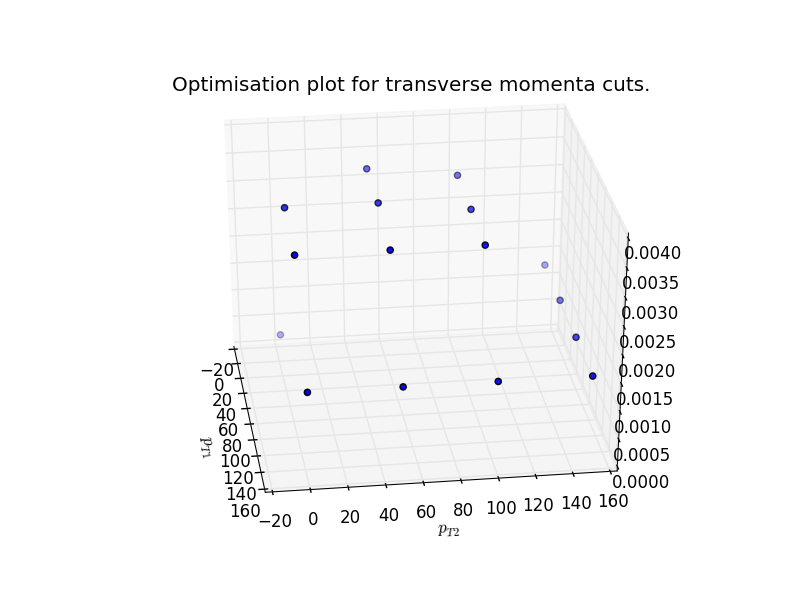
\includegraphics[scale=0.5]{transverse6}
\caption{Statistical signifiance dependence on transverse momenta}
\end{figure}
\subsubsection{Energy}
\begin{figure}
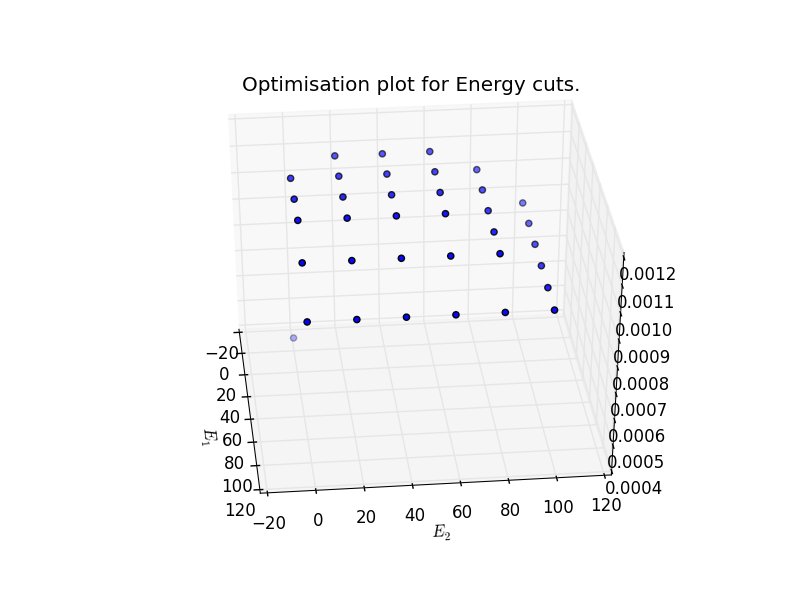
\includegraphics[scale=0.5]{energy6}
\caption{Energy dependence of significance}
\end{figure}
\subsubsection{Azimuthal angle and Pseudo-rapidity}
\begin{figure}
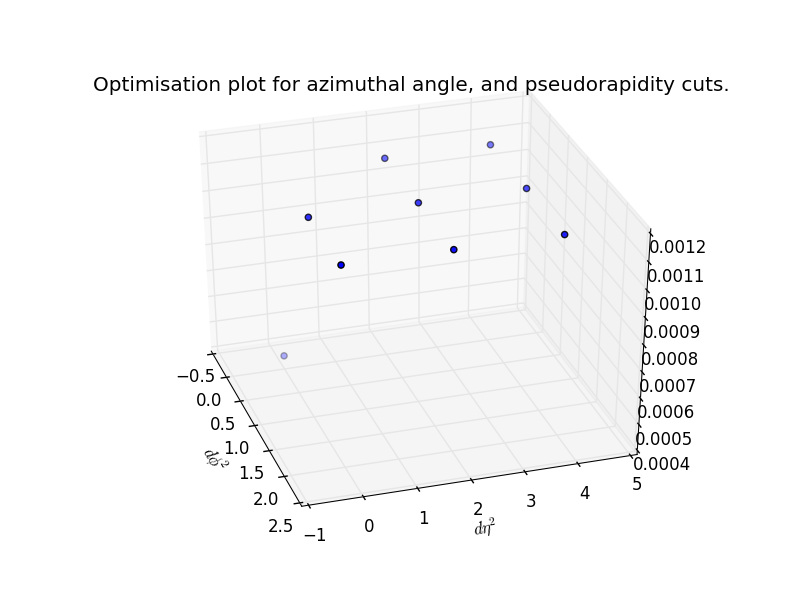
\includegraphics[scale=0.5]{etaphi1}
\caption{Azimuthal and pseudo-rapidity dependence on $\Sigma$}
\end{figure}
%Comment about the inv mass plot before + after optimisation
\subsection{Invariant mass}
%Before
%\begin{figure}
%\includegraphics[scale=0.5]{invariantmassbefore}
%\caption{Invariant mass plot before optimisation}
%\end{figure}
%After
\begin{figure}
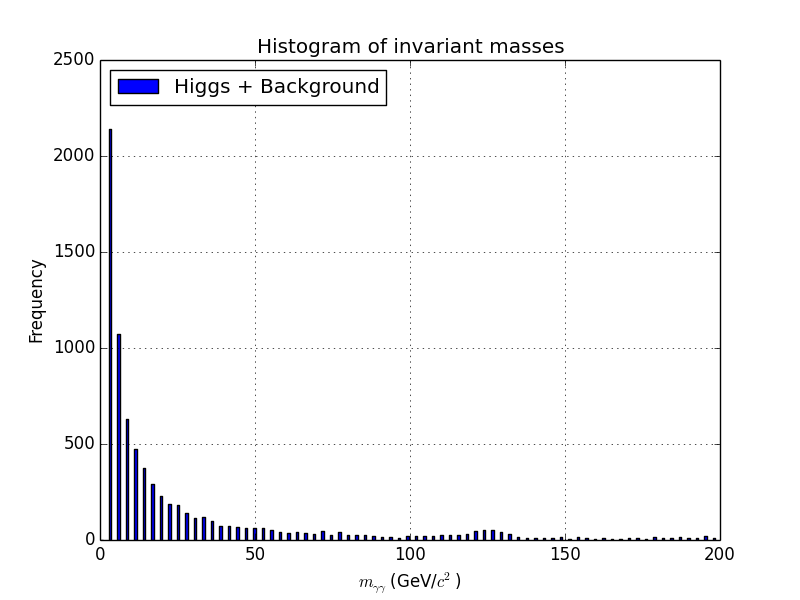
\includegraphics[scale=0.5]{invariantmass1}
\caption{Invariant mass plot after optimisation}
\end{figure}
\section{Conclusion}
The op
\bibliographystyle{plain}
\bibliography{reference}
\appendix
\section{Derivation}
\subsection{Pseudo-rapidity}
\subsection{Derivation of invariant mass}
\section{Code}
\subsection{Parse}
\subsection{Significance}
\subsection{Plot}
\section{Plots}
\subsection{Optimisation}
\subsection{Invariant Mass}
\end{document}
